\documentclass{report}
% Comment the following line to NOT allow the usage of umlauts
\usepackage[utf8]{inputenc}
\usepackage[francais]{babel}
\usepackage{listings}
\usepackage{xcolor}
\usepackage{textcomp}
\usepackage{graphicx}
\pagestyle{plain}
\graphicspath{{DATA/}}
\definecolor{listinggray}{gray}{0.9}
\definecolor{lbcolor}{rgb}{0.9,0.9,0.9}
\lstset{
 backgroundcolor=\color{lbcolor},
 tabsize=4,
 rulecolor=,
 language=matlab,
 basicstyle=\scriptsize,
 upquote=true,
 aboveskip={1.5\baselineskip},
 columns=fixed,
 showstringspaces=false,
 extendedchars=true,
 breaklines=true,
 prebreak = \raisebox{0ex}[0ex][0ex]{\ensuremath{\hookleftarrow}},
 frame=single,
 showtabs=false,
 showspaces=false,
 showstringspaces=false,
 identifierstyle=\ttfamily,
 keywordstyle=\color[rgb]{0,0,1},
 commentstyle=\color[rgb]{0.133,0.545,0.133},
 stringstyle=\color[rgb]{0.627,0.126,0.941},
}

\title{Rapport de TER}
% Start the document
\begin{document}
\maketitle
\newpage
\tableofcontents
\newpage
% Create a new 1st level heading

\part{Présentation du projet}
\chapter{Introduction}
\paragraph{}
L'objectif de ce projet est la réalisation d'un jeu basé sur un modèle multi-agent. L'idée générale du projet est dans la continuité du projet de l'année dernière sur le thème. L'outil utilisé est Unity 3D, un moteur de jeu utilisé dans un grand nombre de réalisation de hautes qualités. Notre projet est utilisable sur Windows et Mac et pourrais être porté sur Android.
Ce projet consiste de réaliser un jeu que l'on peut qualifier de programmeur et de permettre, notamment, à de jeunes personnes de se familiariser avec le monde de la programmation. L'utilisateur pourra donc créer un comportement pour des robots appelé "unité" afin de remplir des objectifs du jeu.
\paragraph{}
Le projet Metabot est un projet modeste réalisé à partir du logiciel Unity 3D par un groupe d'étudiant débutant dans l'utilisation de cet outil. Malgré le peu d'expérience dans la création pure de ce genre de projet, le projet actuel est le fruit d'un travail important et d'une implication entière de toute l'équipe.
Le projet a donc pour unique prétention de communiquer notre amour du jeu vidéo et de la programmation.
\newpage
\chapter{MetaBot: Le mode par défaut}
\section{Principe}
Dans MetaBot, deux à quatre équipes se battent sur un terrain pour les ressources afin de survivre et d'éliminer les autres équipes afin d’être la dernière ne vie. Des ressources apparaissent sur la carte et peuvent etre converti en unité ou en soin.

\newpage
\part{Réalisation du projet}
\newpage

%%%
% PARTIE MOTEUR
%%%
\chapter{Partie "Moteur"}
\section{Phase de conception}
Pour réaliser ce projet, nous avons réalisé une conception basé sur nos connaissances
\section{De l'étude de l'ancien projet à la refonte totale du moteur.}
\subsection{État de l'art de l'ancien projet.}


\subsection{Refont du noyau.}

\section{Réalisation}
\subsection{Sur les unités.}
\subsubsection{Le corps}
\subsubsection{L'esprit}
Afin de pouvoir fonctionner, les unités possede 3 parties distinctes: La gestion des actions possibles, la gestion des perceptions et l'identité propre de l'unité.
\paragraph{Actions.}
Blablabla
\paragraph{Perceptions.}
Blablabla
\paragraph{Identité.}
Blablabla
\section{Fonctionnalités}
\section{Amélioration possible}

\newpage
\chapter{Partie "Graphisme"}

\newpage
\chapter{Partie "Interpreteur"}
repasser sur le texte pour ajouter exemples et illustrations ! 
\section{Présentation et Attente}
La partie "Interpréteur" est la partie la moins visible du projet MetaBot,
mais il s'agit de la partie du projet servant de clé de voute du jeu.
Comme dit plus tôt, la particularité de MetaBot est que le joueur, qui pourra être considéré comme le programmeur, va préparer en amont une cohésion d'équipe à travers le comportement et va pouvoir lancer un match contre une autre équipe, afin d'évaluer quel comportement sera le meilleur.
L'interpreteur permet de faire la liaison entre l'éditeur du comportement ou l'utilisateur va développer son comportement, en utilisant un ensemble de d'instructions que nous avons prédéfinies  et la partie moteur, ou le fonctionnement des unités est inscrit, ainsi que les différents modes de jeux.
\paragraph{}
Le langage et l'ensemble des instructions nécessaires est alimenté par l'équipe Game Design qui nous a donné des exemples de messages ou de spécificités du langage qui pourrait être nécessaire. On pouvait ensuite tous en discuter en pesant le pour et le contre, afin de définir si la fonctionnalité allait être mise en place , et de quelle façon.
\section{Etude de l'ancien projet et récupération de ce qui est utile}
Au départ, il a été nécessaire de remettre en place un outil permettant de récupérer un comportement, qui était uniquement graphique, dans l'éditeur afin de pouvoir le renvoyer à la partie Moteur, pour que l'ensemble des unités puissent l'exécuter.
Nous avons pris connaissance de ce que l'ancien groupe avait mis en place et avons trié ce qui nous semblait correspondre à notre version du projet.
Il était obligatoire d'écrire le comportement récupéré de l'éditeur dans un fichier, afin de le récupérer , pouvoir le modifier , le déplacer , et le conserver pour plusieurs parties.
La solution mise en place par l'ancien groupe pour le stockage, qui était d'utiliser un fichier XML correspondait parfaitement à notre besoin, car la syntaxe et l'organisation en nœuds de ce genre de fichiers, permettait une récupération simple et claire des instructions. Nous avons ainsi pu récupérer une bonne partie de leur système d'écriture et de lecture de leur projet, tout en adaptant l'autre partie à nos besoins.
\paragraph{}
\newpage
La partie organisant les instructions à été complètement supprimée, et nous avons repensé un système plus générique et plus compréhensible pour les groupes qui vont récupérer ce projet plus tard.
\section{Conception et implémentation}
La construction des Instructions des unités dans la partie Interpréteur a grandement été facilitée et la liaison des instructions avec leur exécution a été décalée dans le moteur. Ainsi on ne manipule que des chaînes de caractères lors de l'accès dans le fichier, et le moteur effectue la liaison avec une structure de "Delegate" comme expliqué plus haut, rajoutant beaucoup de généricité au projet.
D'un point de vue de la sécurité, celle-ci a été décalée dans l'éditeur du comportement, afin de ne pas traiter des comportements erronés , mais prévenir a l'avance et même empêcher les erreurs d'apparaitre.
\paragraph{}
Le but de l'interpréteur était de traiter des fichiers de ce type :
\begin{lstlisting}[frame=single]
<behavior>
  <teamName>Default Team</teamName>
  <unit name="Explorer">
    <instruction>
    </instruction>
  </unit>
  <unit name="Base">
  </unit>
  <unit name="Light">
  </unit>
  <unit name="Heavy">
  </unit>
</behavior>
\end{lstlisting}
Ainsi nous avons 1 fichier par équipe écrite par l'utilisateur, chacun détaillant le comportement de chaque unité sous la même forme :
\begin{lstlisting}[frame=single]
<behavior>
  <teamName>Default Team</teamName>
  <unit name="Explorer">
 <instruction>
      <parameters>
        <PERCEPT_ENEMY />
      </parameters>
      <message>
        <ACTN_MESSAGE_HELP>
          <Light />
        </ACTN_MESSAGE_HELP>
      </message>
      <actions>
        <ACTION_MOVE />
      </actions>
    </instruction>
    <instruction>
    </instruction>
  </unit>
</behavior>
\end{lstlisting}
Le comportement d'une unité est une suite d'instructions, dont l'ordre est très important. La hiérarchie va déterminer la priorité qu'aura l'action sur le tick. Ainsi l'action la plus prioritaire dont les conditions sont acceptées sera l'action effectuée sur ce tick.
Chaque instruction est toujours organisée de la même façon :
- Une liste de conditions à remplir pour que l'instruction soit considéré comme acceptée
- Une liste d'actions qui ne terminent pas l'action, appelées Actions non terminales, mais qui peuvent être les messages partagés entre les unités par exemple. Ces actions non terminales seront exécutés avant :
- L'action terminale, qui va être exécutée à la fin du tick pour l'ensemble des unités et va être l'action qui va être "physiquement" fait par l'unité, par exemple : Avancer, Tirer, Récupérer ou donner une ressource,Se soigner , ...
\paragraph{}
Comme dit précédemment, l'interpréteur relie les 2 parties majeures du projet.
Ainsi, une fonction permet de transformer un fichier ".wbt" (format des équipes WarBot) vers un comportement d'équipe utilisable par l'équipe moteur, et une fonction permettant la transformation d'un comportement récupéré de l'éditeur graphique vers un fichier XML, pour sa sauvegarde.
\newpage
\paragraph{}
Un nouveau travail d'interprétation a vite été ressenti dans le projet. En effet, le jeu étant destiné à aider les jeunes à appréhender la programmation, une traduction française était nécessaire.
Toujours dans l'idée de rester générique, un traducteur a été mis en place et attaché à l'ensemble des textes qui seront affichés à l'utilisateur.
\paragraph{}
%pas clair a changer
La traduction fonctionne ainsi :
Un premier script s'occupe de vérifier la langue qui doit être utilisée dans le fichier de configuration du jeu et va charger en mémoire un fichier  de traductions : 

Le fichier va être parcouru, et un ensemble de couples clé,valeurs vont être récupérés , la clé correspondant à la valeur initiale d'un bouton/ texte affiché, la valeur étant la traduction qu'il faudra affiché à la place de la clé.

Ce script est ainsi rattaché au "GameManager" , un objet Unity qui n'est pas détruit lorsque l'on change de scène. Ainsi les traductions sont conservées lorsqu'on passe de l'éditeur au menu principal , du menu principal aux cartes de jeu, ...
\paragraph{}
Un second script est lui attaché à tous les Objets du jeu qui vont devoir être traduits. Celui-ci va , à la création de l'objet auquel il est rattaché, chercher la langue actuellement affichée, récupérer comme clé le texte original de l'objet auquel le script est affilié, et va stocker la traduction, et l'afficher à l utilisateur.
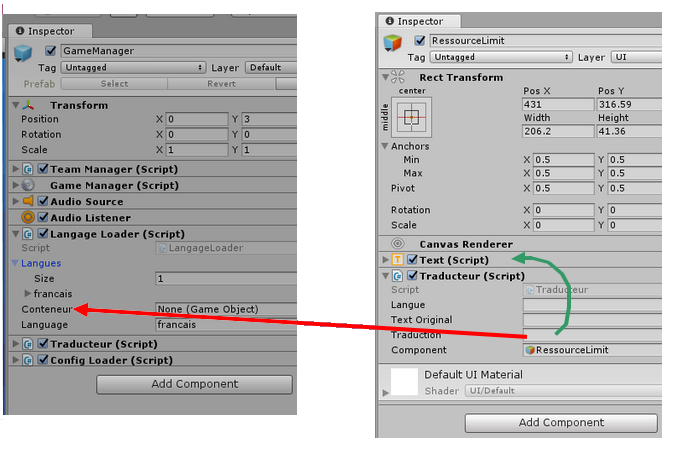
\includegraphics{traducteur2.png}

En Runtime, si la langue est changée dans les paramètres du jeu, les script de traduction des objets vont mettre à jour leur langue, et récupérer la nouvelle traduction dans le "GameManager".
\paragraph{}
La traduction est aussi disponible sans rattacher un script "Traducteur" à un Objet de la scène.
En effet, il y a beaucoup de situations ou on ne peut pas rattacher ce script. On peut récupérer la traduction via le champ "traduction" du traducteur après l'avoir instancié dans un script externe, et l'afficher ou l'utiliser à la place de ce qu'on l'on voulait traduire.
\paragraph{}
La récupération de la langue du projet se fait à travers un fichier paramètre à la création du Traducteur, que ce soit dans la scène ou dans un script. 
Celle-ci est stockée en clair dans un fichier de paramétrage : 
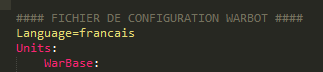
\includegraphics{fichierconfig.png}
Mais ce fichier est caché, à moins de connaître sa position dans la hiérarchie et de devoir redémarrer le jeu pour changer la langue, 2 boutons sont dans les paramètres pour passer en Français ou en Anglais. Si le besoin de nouvelles langues se fait sentir dans le futur, il sera toujours possible de transformer ces boutons en un "DropDown" , un menu déroulant, afin de pouvoir sélectionner autant de langues que disponible.
\paragraph{}
L'ajout de traductions est externe au jeu. 
Dans les fichiers du jeu , on retrouve un dossier contenant ces traductions,sous formes de fichier représentant chacun une langue.
Une traduction est simplement une ligne du fichier mettant en relation une clé et sa traduction.
Le rajout d'une langue est simple est totalement simple et générique :
On ajoute un fichier ayant le nom de la langue que l'on souhaite, et qui doit obligatoirement implémenter l'ensemble des clés présentes dans les autres fichiers, ou dans le fichier "example" mis à disposition.

Voici à quoi ressemble les fichiers de traduction :
\begin{lstlisting}[language=XML]
# Percepts
	PERCEPT_ALLY=PERCEPT_ALLIE_A_PORTEE
	FALSE_PERCEPT_ALLY=PERCEPT_AUCUN_ALLIE_A_PORTEE
	PERCEPT_BLOCKED=PERCEPT_EST_BLOQUE
	FALSE_PERCEPT_BLOCKED=PERCEPT_N'EST_PAS_BLOQUE
	PERCEPT_IS_RELOADED=PERCEPT_EST_RECHARGE
	FALSE_PERCEPT_IS_RELOADED=PERCEPT_N'EST_PAS_RECHARGE
	PERCEPT_IS_NOT_RELOADED=PERCEPT_PAS_RECHARGE
	FALSE_PERCEPT_IS_NOT_RELOADED=PERCEPT_EST_RECHARGE
# Map en jeu 
	Recommencer=Recommencer
	Quitter=Quitter
	Health : =Vie : 
	Bag : =Sac : 
	Heading : =Orientation : 
	Contract :=Contrat :
\end{lstlisting}

On a donc ici bien le système de clé / valeur expliqué plus haut. 
On peut voir que le caractère séparateur est le caractère ' = ' , au départ nous utilisions le caractère ' : ' , mais il y a eu des conflits puisque les textes affichés sur l'interface utilisateur contiennent aussi les ':'.
Il est possible que le caractère ' = ' pose problème au bout d'un moment, si jamais des traductions ajoutées ultérieurement le contiennent. Il faudra donc simplement faire une recherche "Trouver et Remplacer" dans les fichiers de traduction, et changer un seul caractère dans le code du Parser des fichiers de traductions. 

\paragraph{}

La traduction dupliquée de chaque texte comme vue dans la partie "Percepts" de l'exemple plus haut à laquelle on rajoute un "FALSE_" provient du fait que les conditions et perceptions qui sont traitées dans le jeu peuvent être mises au négatif. Par exemple, si le comportement d'une unité de mon équipe cherche à savoir si cette unité à "un contrat d'élimination en cours" lorsqu'elle reçoit le message demandant de l'aide depuis la base, il est tout à fait possible que l'on cherche à vérifier que l'on a aucun contrat d'élimination pour pouvoir en accepter un nouveau.
Au lieu de dupliquer les conditions dans le code , il a été préféré de pouvoir les rendre négatives.


\newpage
\chapter{Partie "Game Design"}

\newpage
\part{L'avenir du projet}
\chapter{Amélioration possible}

% Uncomment the following two lines if you want to have a bibliography
%\bibliographystyle{alpha}
%\bibliography{document}

\end{document}
